\section{Analyse et conception}

\subsection{Partie 1 -- Registre à décalage 4 bits}

Le registre est formé de 4 cellules identiques, une par bit. Chaque cellule contient une bascule D (horloge \texttt{clock\_i}, reset asynchrone \texttt{reset\_i}) précédée d'un multiplexeur 2 vers 1 commandé par \texttt{en\_sh\_i} :
\begin{itemize}
	\item \texttt{en\_sh\_i} = 1 : la cellule reçoit le bit de la cellule de gauche (décalage à droite). La première cellule (bit 3) reçoit \texttt{ser\_r\_i} ;
	\item \texttt{en\_sh\_i} = 0 : la cellule reçoit sa propre sortie Q et conserve son bit.
\end{itemize}
\[
D_n = \overline{\texttt{en\_sh\_i}} \cdot Q_n + \texttt{en\_sh\_i} \cdot Q_{n+1}, \qquad \text{avec } Q_4 = \texttt{ser\_r\_i}
\]

\subsection{Partie 2 -- Registre à décalage 8 bits}

\begin{schema}
	\centering
	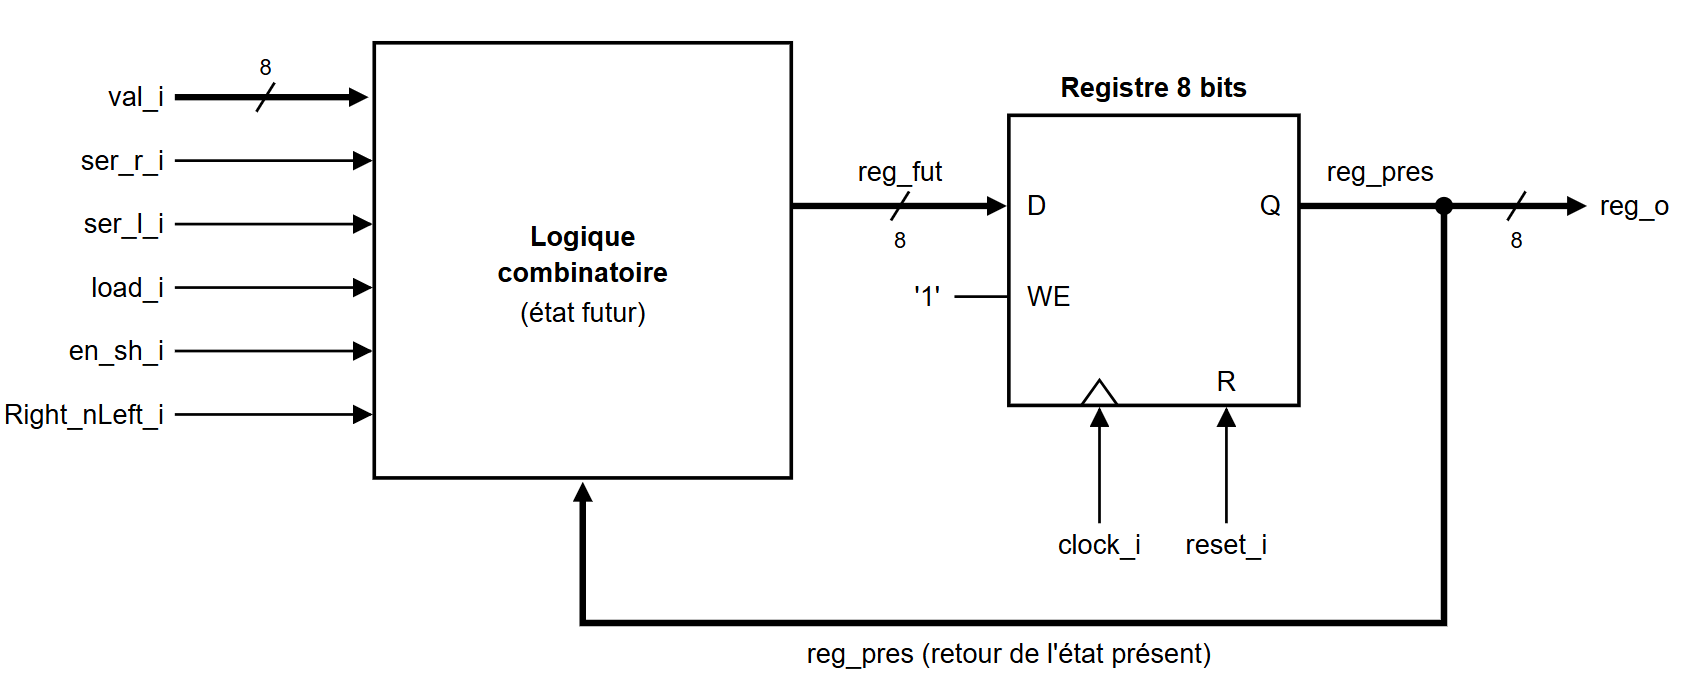
\includegraphics[width=\textwidth]{./images/analyse-partie2.png}
	\caption{Partie 2, schéma bloc, registre à décalage 8 bits}
	\label{fig:analyse_p2}
\end{schema}

Le registre suit la structure d'un système séquentiel synchrone (voir \emph{\underline{Schéma~\ref{fig:analyse_p2}}}) : un bloc combinatoire calcule l'état futur \texttt{reg\_fut} à partir de l'état présent \texttt{reg\_pres} et des commandes, et un registre parallèle/parallèle de 8 bits le mémorise à chaque flanc montant de \texttt{clock\_i}. Son entrée WE est fixée à 1 : le registre est chargé à chaque flanc, c'est donc la logique qui doit recopier \texttt{reg\_pres} lorsque la valeur doit être conservée.

Le bloc combinatoire est décrit par la table des fonctions synchrones (voir \emph{\underline{Tableau~\ref{tab:fonctions_p2}}}), où le cas le plus prioritaire est en haut. Le chargement parallèle passe avant tout le reste, sinon, \texttt{en\_sh\_i} autorise le décalage, dont le sens est donné par \texttt{Right\_nLeft\_i}.

\begin{table}[H]
	\centering
	\small
	\setlength{\tabcolsep}{4.5pt}
	\begin{tabular}{@{}cccll@{}}
		\toprule
		\texttt{load\_i} & \texttt{en\_sh\_i} & \texttt{Right\_nLeft\_i} & \textbf{Fonction} & \texttt{reg\_fut(7..0)} \\
		\midrule
		1 & - & - & Chargement parallèle & \texttt{val\_i(7..0)} \\
		0 & 1 & 1 & Décalage à droite & \texttt{ser\_r\_i \& reg\_pres(7..1)} \\
		0 & 1 & 0 & Décalage à gauche & \texttt{reg\_pres(6..0) \& ser\_l\_i} \\
		0 & 0 & - & Maintien & \texttt{reg\_pres(7..0)} \\
		\bottomrule
	\end{tabular}
	\caption{Partie 2, table des fonctions synchrones, bloc état futur}
	\label{tab:fonctions_p2}
\end{table}

\newpage

\subsection{Partie 3 -- Chenillard}

Le chenillard charge un pattern de 8 bits (\texttt{pattern\_i}, avec \texttt{load\_i}) et le fait tourner d'une position à chaque flanc montant lorsque \texttt{en\_i} = 1, à droite si \texttt{right\_nLeft\_i} = 1, à gauche sinon. La rotation est cyclique : le bit qui sort d'un côté revient de l'autre (voir \emph{\underline{Figure~\ref{fig:exemple_p3}}}).

\begin{figure}[H]
	\centering
	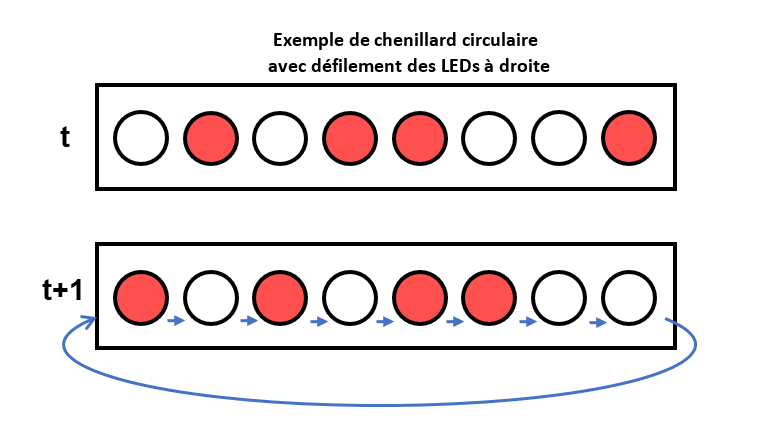
\includegraphics[width=0.7\textwidth]{./images/realisation-partie3-exemple.png}
	\caption{Partie 3, exemple de chenillard circulaire avec rotation à droite (donnée du laboratoire)}
	\label{fig:exemple_p3}
\end{figure}

Le registre de la partie 2 sait déjà charger et décaler. Il suffit donc de reboucler les bits extrêmes sur les entrées série :
\begin{itemize}
	\item \texttt{reg\_o(0)} sur \texttt{ser\_r\_i} : en rotation à droite, le bit 0 revient sur le bit 7 ;
	\item \texttt{reg\_o(7)} sur \texttt{ser\_l\_i} : en rotation à gauche, le bit 7 revient sur le bit 0.
\end{itemize}
